\documentclass[11pt,compress,t,notes=noshow, xcolor=table]{beamer}
\usepackage[]{graphicx}\usepackage[]{color}
% maxwidth is the original width if it is less than linewidth
% otherwise use linewidth (to make sure the graphics do not exceed the margin)
\makeatletter
\def\maxwidth{ %
  \ifdim\Gin@nat@width>\linewidth
    \linewidth
  \else
    \Gin@nat@width
  \fi
}
\makeatother

\newcommand{\citebutton}[2]{%
\beamergotobutton{\href{#2}{#1}}%
}

\newcommand{\blu}[1]{\textcolor{blue}{#1}}
\newcommand{\org}[1]{\textcolor{orange}{#1}}
\newcommand{\ques}{\textbf{\textcolor{red}{Question:  }}}
\newcommand{\questionssofar}{\begin{frame}\frametitle{Any questions?}\end{frame}}

\newcommand\warning{%
 \makebox[1.4em][c]{%
 \makebox[0pt][c]{\raisebox{.1em}{\scriptsize!}}%
 \makebox[0pt][c]{\color{red}\normalsize$\bigtriangleup$}}}%

\definecolor{fgcolor}{rgb}{0.345, 0.345, 0.345}
\newcommand{\hlnum}[1]{\textcolor[rgb]{0.686,0.059,0.569}{#1}}%
\newcommand{\hlstr}[1]{\textcolor[rgb]{0.192,0.494,0.8}{#1}}%
\newcommand{\hlcom}[1]{\textcolor[rgb]{0.678,0.584,0.686}{\textit{#1}}}%
\newcommand{\hlopt}[1]{\textcolor[rgb]{0,0,0}{#1}}%
\newcommand{\hlstd}[1]{\textcolor[rgb]{0.345,0.345,0.345}{#1}}%
\newcommand{\hlkwa}[1]{\textcolor[rgb]{0.161,0.373,0.58}{\textbf{#1}}}%
\newcommand{\hlkwb}[1]{\textcolor[rgb]{0.69,0.353,0.396}{#1}}%
\newcommand{\hlkwc}[1]{\textcolor[rgb]{0.333,0.667,0.333}{#1}}%
\newcommand{\hlkwd}[1]{\textcolor[rgb]{0.737,0.353,0.396}{\textbf{#1}}}%
\let\hlipl\hlkwb

\usepackage{framed}
\makeatletter
\newenvironment{kframe}{%
 \def\at@end@of@kframe{}%
 \ifinner\ifhmode%
  \def\at@end@of@kframe{\end{minipage}}%
  \begin{minipage}{\columnwidth}%
 \fi\fi%
 \def\FrameCommand##1{\hskip\@totalleftmargin \hskip-\fboxsep
 \colorbox{shadecolor}{##1}\hskip-\fboxsep
     % There is no \\@totalrightmargin, so:
     \hskip-\linewidth \hskip-\@totalleftmargin \hskip\columnwidth}%
 \MakeFramed {\advance\hsize-\width
   \@totalleftmargin\z@ \linewidth\hsize
   \@setminipage}}%
 {\par\unskip\endMakeFramed%
 \at@end@of@kframe}
\makeatother

\definecolor{shadecolor}{rgb}{.97, .97, .97}
\definecolor{messagecolor}{rgb}{0, 0, 0}
\definecolor{warningcolor}{rgb}{1, 0, 1}
\definecolor{errorcolor}{rgb}{1, 0, 0}
\newenvironment{knitrout}{}{} % an empty environment to be redefined in TeX

\usepackage{alltt}
\newcommand{\SweaveOpts}[1]{}  % do not interfere with LaTeX
\newcommand{\SweaveInput}[1]{} % because they are not real TeX commands
\newcommand{\Sexpr}[1]{}       % will only be parsed by R
\newcommand{\xmark}{\ding{55}}%


\usepackage[english]{babel}
\usepackage[utf8]{inputenc}

\usepackage{dsfont}
\usepackage{verbatim}
\usepackage{amsmath}
\usepackage{amsfonts}
\usepackage{amssymb}
\usepackage{bm}
\usepackage{csquotes}
\usepackage{multirow}
\usepackage{longtable}
\usepackage{booktabs}
\usepackage{enumerate}
\usepackage[absolute,overlay]{textpos}
\usepackage{psfrag}
\usepackage{algorithm}
\usepackage{algpseudocode}
\usepackage{eqnarray}
\usepackage{arydshln}
\usepackage{tabularx}
\usepackage{placeins}
\usepackage{tikz}
\usepackage{setspace}
\usepackage{colortbl}
\usepackage{mathtools}
\usepackage{wrapfig}
\usepackage{bm}
\usepackage{amsmath}
\usepackage{pifont}

\usetikzlibrary{shapes.multipart,shapes,arrows,automata,positioning,calc,chains,trees, shadows}
\tikzset{
  %Define standard arrow tip
  >=stealth',
  %Define style for boxes
  punkt/.style={
    rectangle,
    rounded corners,
    draw=black, very thick,
    text width=6.5em,
    minimum height=2em,
    text centered},
  % Define arrow style
  pil/.style={
    ->,
    thick,
    shorten <=2pt,
    shorten >=2pt,}
}

\tikzstyle{vec}=[draw, rectangle, fill = white, minimum width=5mm, minimum height=1cm, inner sep = 2pt]

\usepackage{subfig}

% Defines macros and environments
\usepackage{../../style/lmu-lecture}


\let\code=\texttt
\let\proglang=\textsf

\setkeys{Gin}{width=0.9\textwidth}

\setbeamertemplate{frametitle}{\expandafter\uppercase\expandafter\insertframetitle}

\usepackage{bbm}
% basic latex stuff
\newcommand{\pkg}[1]{{\fontseries{b}\selectfont #1}} %fontstyle for R packages
\newcommand{\lz}{\vspace{0.5cm}} %vertical space
\newcommand{\dlz}{\vspace{1cm}} %double vertical space
\newcommand{\oneliner}[1] % Oneliner for important statements
{\begin{block}{}\begin{center}\begin{Large}#1\end{Large}\end{center}\end{block}}


%new environments
\newenvironment{vbframe}  %frame with breaks and verbatim
{
 \begin{frame}[containsverbatim,allowframebreaks]
}
{
\end{frame}
}

\newenvironment{vframe}  %frame with verbatim without breaks (to avoid numbering one slided frames)
{
 \begin{frame}[containsverbatim]
}
{
\end{frame}
}

\newenvironment{blocki}[1]   % itemize block
{
 \begin{block}{#1}\begin{itemize}
}
{
\end{itemize}\end{block}
}

\newenvironment{fragileframe}[2]{  %fragile frame with framebreaks
\begin{frame}[allowframebreaks, fragile, environment = fragileframe]
\frametitle{#1}
#2}
{\end{frame}}


\newcommand{\myframe}[2]{  %short for frame with framebreaks
\begin{frame}[allowframebreaks]
\frametitle{#1}
#2
\end{frame}}

\newcommand{\remark}[1]{
  \textbf{Remark:} #1
}


\newenvironment{deleteframe}
{
\begingroup
\usebackgroundtemplate{
\includegraphics[width=\paperwidth,height=\paperheight]{../style/color/red.png}}
 \begin{frame}
}
{
\end{frame}
\endgroup
}
\newenvironment{simplifyframe}
{
\begingroup
\usebackgroundtemplate{
\includegraphics[width=\paperwidth,height=\paperheight]{../style/color/yellow.png}}
 \begin{frame}
}
{
\end{frame}
\endgroup
}\newenvironment{draftframe}
{
\begingroup
\usebackgroundtemplate{
\includegraphics[width=\paperwidth,height=\paperheight]{../style/color/green.jpg}}
 \begin{frame}
}
{
\end{frame}
\endgroup
}
% https://tex.stackexchange.com/a/261480: textcolor that works in mathmode
\makeatletter
\renewcommand*{\@textcolor}[3]{%
  \protect\leavevmode
  \begingroup
    \color#1{#2}#3%
  \endgroup
}
\makeatother





\input{../../latex-math/basic-math.tex}
\input{../../latex-math/basic-ml.tex}

\newcommand{\blu}[1]{\textcolor{blue}{#1}}
\newcommand{\org}[1]{\textcolor{orange}{#1}}
\newcommand{\ques}{\textbf{\textcolor{red}{Question:  }}}
\newcommand{\questionssofar}{\begin{frame}\frametitle{Any questions?}\end{frame}}

\newcommand\warning{%
 \makebox[1.4em][c]{%
 \makebox[0pt][c]{\raisebox{.1em}{\scriptsize!}}%
 \makebox[0pt][c]{\color{red}\normalsize$\bigtriangleup$}}}%

\newcommand{\titlefigure}{figure/transformer.png}
\newcommand{\learninggoals}{
\item Understand BPE
\item Understand the Transformer Encoder + Decoder
\item Understand how they are connected
\item Understand the limitations for long sequences}

\title{Transformer}
% \author{Bernd Bischl, Christoph Molnar, Daniel Schalk, Fabian Scheipl}
\institute{\href{https://slds-lmu.github.io/lecture_dl4nlp/}{slds-lmu.github.io/lecture\_dl4nlp}}
\date{}

\begin{document}
\lecturechapter{The Encoder}
\lecture{Deep Learning for NLP}

% ------------------------------------------------------------------------------

\begin{vbframe}{The Transformer architecture}

\begin{center}
\begin{tikzpicture}[->, >=stealth, thick, font=\scriptsize]
\node (transformer) at (0,0) {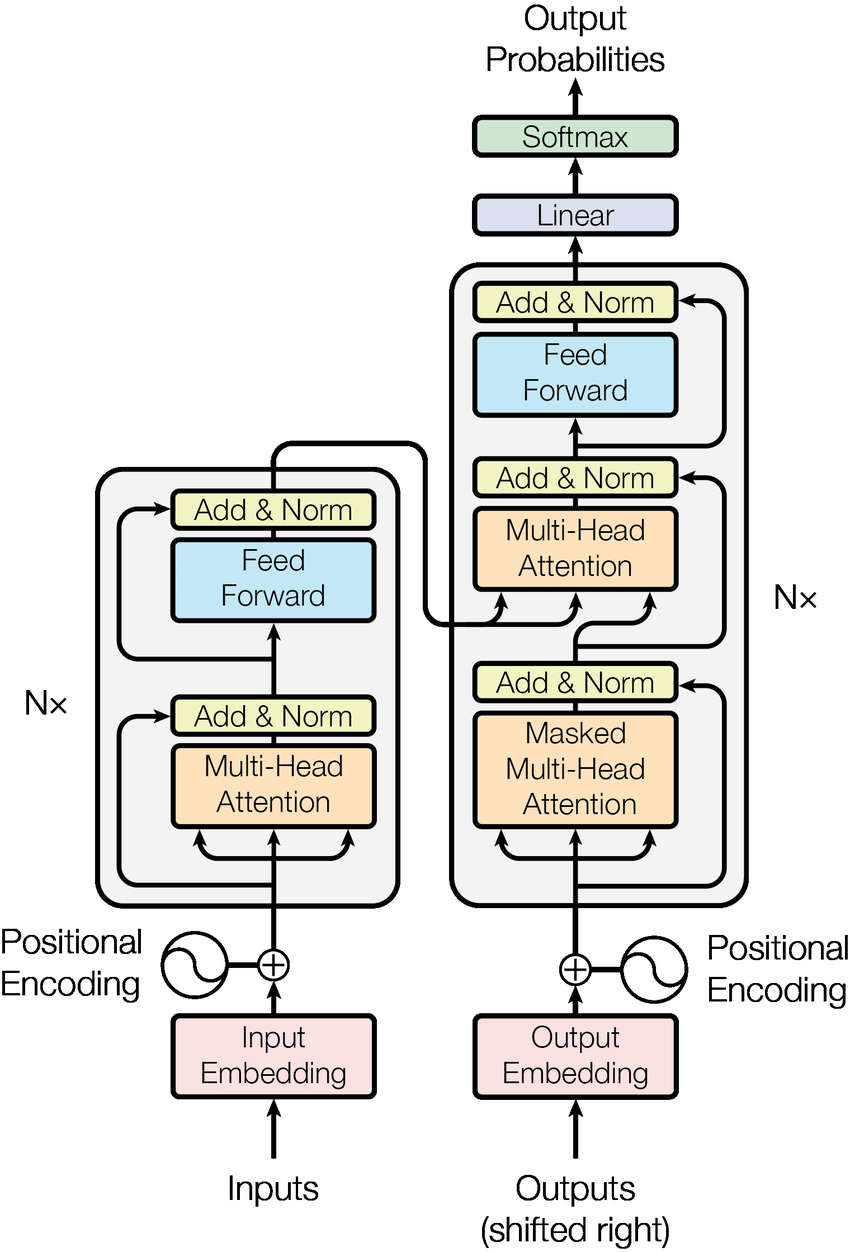
\includegraphics[width=.4\textwidth]{figure/transformer.png}};
\node (enc) [left=2mm of transformer, rotate=90] {encoder};
\node (dec) [right=2mm of transformer, rotate=270] {decoder};
\node (x) [above left=1cm of transformer.south west] {$X$ (source)};
\node (y) [above right=1cm of transformer.south east] {$Y$ (target)};
\draw (x) -- ([yshift=5mm, xshift=1cm] transformer.south west);
\draw (y) -- ([yshift=5mm, xshift=-1cm] transformer.south east);
\node (nll) [draw, circle] at ([yshift=-5mm] transformer.north east) {NLL};
\draw [bend right=55] (y.north east) to (nll);
\draw ([xshift=-1cm, yshift=-5mm] transformer.north east) to (nll);
\node at (-3, 2) [align=left] {(For simpler problems (e.g., \\ classification, tagging), \\ you would simply use \\ the encoder.)};
\end{tikzpicture}
\end{center}
{\tiny Figure from Vaswani et al. 2017: Attention is all you need}

\end{vbframe}

% ------------------------------------------------------------------------------

\begin{vbframe}{Attention in the Transformer}

\vfill

\begin{itemize}
\item We can use attention on many different ``things'', including: 
\begin{itemize}
\item The pixels of images
\item The nodes of knowledge graphs
\item The words of a vocabulary
\end{itemize}
\item Here, we focus on scenarios where the query, key and value vectors represent tokens (e.g., words, characters, etc.) in sequences (e.g., sentences, paragraphs, etc.).
\end{itemize}

\vfill

\end{vbframe}

% ------------------------------------------------------------------------------

\begin{vbframe}{Attention in the Transformer}

\vfill

\textbf{Cross-attention:}
\begin{itemize}
\item Let $X = (x_1 \ldots x_{J_x}), Y = (y_1 \ldots y_{J_y})$ be two sequences (e.g., source and target in a sequence-to-sequence problem)
\item The query vectors represent tokens in $Y$ and the key/value vectors represent tokens in $X$ (``$Y$ attends to $X$'')
\end{itemize}
\textbf{Self-attention:}
\begin{itemize}
\item There is only one sequence $X = (x_1 \ldots x_J)$
\item The query, key and value vectors represent tokens in $X$ (``$X$ attends to itself'')
\end{itemize}

\vfill

\end{vbframe}

% ------------------------------------------------------------------------------

\begin{vbframe}{Self-Attention formalized}

\vfill

\begin{itemize}
\item Let $\vec X \in \mathbb{R}^{J_x \times d_x}$ be a representation of $X$ (e.g., stacked word embeddings, or the outputs of a previous layer)
\item Let $\theta = \{\vec W^{(q)} \in \mathbb{R}^{d_x \times d_q}, \vec W^{(k)} \in \mathbb{R}^{d_x \times d_k}, \vec W^{(v)} \in \mathbb{R}^{d_x \times d_v}\}$ be trainable weight matrices
\item We transform $\vec X$ into a matrix of query vectors:
$$ \vec Q = \vec X \vec W^{(q)} $$
\item And we transform $\vec X$ into matrices of key and value vectors:
$$ \vec K = \vec X \vec W^{(k)} ; \qquad \vec V =  \vec X \vec W^{(v)}$$
\end{itemize}

\vfill

\end{vbframe}

% ------------------------------------------------------------------------------

\begin{vbframe}{Can self-attention model word order?}

\vfill

\begin{itemize}
	\item Our model consists of a self-attention layer on top of a simple word embedding lookup layer. (For simplicity, we only consider one head, but this applies to multi-head attention as well.)
	\item Let $\blu{X^{(1)}}$, $\org{X^{(2)}}$ be two sentences of the same length $J$, which contain the same words in a different order
	\item Example: \blu{``john loves mary''} vs. \org{``mary loves john''}
\end{itemize}
\begin{center}
	
\includegraphics[width=.6\textwidth]{figure/mary_loves_john}
\end{center}

\vfill

\end{vbframe}

% ------------------------------------------------------------------------------

\begin{vbframe}{Can self-attention model word order?}

\vfill

\begin{itemize}
\item Definition of $\vec o_j$:
$$\vec o_j = \sum_{j'=1}^J \alpha_{j,j'} \vec v_{j'}$$
\item Since addition is commutative, and the permutation is bijective, it is sufficient to show that:
$$\forall_{j \in \{1,...,J\}, j' \in \{1,...,J\}} \blu{\alpha^{(1)}_{j,j'} \vec v^{(1)}_{j'}} = \org{\alpha^{(2)}_{g_j,g_{j'}} \vec v^{(2)}_{g_{j'}}}$$
\item Step 1: Let's show that $\forall_{j} \blu{\vec v^{(1)}_{j}} = \org{\vec v^{(2)}_{g_{j}}}$
\item Definition of $\vec v_j$:
$$\vec v_j = \vec W^{(v)T} \vec x_j$$
\item Then:
$$\blu{\vec x^{(1)}_{j}} = \org{\vec x^{(2)}_{g_{j}}} \implies \vec W^{(v)T} \blu{\vec x^{(1)}_{j}} = \vec W^{(v)T} \org{\vec x^{(2)}_{g_{j}}} \implies \blu{\vec v^{(1)}_j} = \org{\vec v^{(2)}_{g_j}}$$
\end{itemize}

\vfill

\end{vbframe}

% ------------------------------------------------------------------------------

\begin{vbframe}{Can self-attention model word order?}

\vfill

\begin{itemize}
\item Step 2: Let's show that $\forall_{j \in \{1,...,J\}, j' \in \{1,...,J\}} \blu{\alpha^{(1)}_{j, j'}} = \org{\alpha^{(2)}_{g_j, g_{j'}}}$
\item Definition of $\alpha_{j,j'}$:
$$\alpha_{j,j'} = \frac{\mathrm{exp}(e_{j,j'})}{\sum_{j''=1}^J \mathrm{exp}(e_{j,j''})}$$
\item Since the sum in the denominator is commutative, and the permutation is bijective, it is sufficient to show that
$$\forall_{j \in \{1,...,J\}, j' \in \{1,...,J\}} \blu{e^{(1)}_{j,j'}} = \org{e^{(2)}_{g_j, g_{j'}}}$$
\end{itemize}

\vfill

\end{vbframe}

% ------------------------------------------------------------------------------

\begin{vbframe}{Can self-attention model word order?}

\vfill

\begin{itemize}
\item Definition of $e_{j,j'}$:
$$e_{j,j'} = \frac{1}{\sqrt{d_k}} \vec q_{j}^T \vec k_{j'} = \frac{1}{\sqrt{d_k}} (\vec W^{(q)T} \vec x_{j})^T (\vec W^{(k)T} \vec x_{j'})$$
\item Then:
$$
\begin{aligned}
& \blu{\vec x^{(1)}_j} = \org{\vec x^{(2)}_{g_j}} \land \blu{\vec x^{(1)}_{j'}} = \org{\vec x^{(2)}_{g_{j'}}} \\
\implies{} & \vec W^{(q)T} \blu{\vec x^{(1)}_j} = \vec W^{(q)T} \org{\vec x^{(2)}_{g_j}} \land \vec W^{(k)T} \blu{\vec x^{(1)}_{j'}} = \vec W^{(k)T} \org{\vec x^{(2)}_{g_{j'}}} \\
\implies{} & \blu{\vec q^{(1)}_j} = \org{\vec q^{(2)}_{g_j}} \land \blu{\vec k^{(1)}_{j'}} = \org{\vec k^{(2)}_{g_{j'}}} \\
\implies{} & \blu{\vec q^{(1)T}_j \vec k^{(1)}_{j'}} = \org{\vec q^{(2)T}_{g_j} \vec k^{(2)}_{g_{j'}}} \\
\implies{} & \frac{1}{\sqrt{d_k}} \blu{\vec q^{(1)T}_j \vec k^{(1)}_{j'}} =  \frac{1}{\sqrt{d_k}}  \org{\vec q^{(2)T}_{g_j} \vec k^{(2)}_{g_{j'}}} \\
\implies & \blu{e^{(1)}_{j,j'}} = \org{e^{(2)}_{g_j, g_{j'}}}
\end{aligned}
$$
\end{itemize}

\vfill

\end{vbframe}

% ------------------------------------------------------------------------------

\begin{vbframe}{Can self-attention model word order?}

\vfill

\begin{itemize}
\item So, $\forall_j \blu{\vec o^{(1)}_j} = \org{\vec o^{(2)}_{g_j}}$
\item In other words: The representation of \blu{mary} is identical to that of \org{mary}, and the representation of \blu{john} is identical to that of \org{john}
\item \ques Can the other layers in the Transformer architecture (feed-forward net, layer normalization) help with the problem?
\begin{itemize}
\item No, because they are apply the same function to all positions.
\end{itemize}
\item \ques Would it help to apply more self-attention layers?
\begin{itemize}
\item No. Since the representations of identical words are still identical in $\vec O$, the next self-attention layer will have the same problem.
\end{itemize}
\item So... does that mean the Transformer is unusable?
\item Luckily not. We just need to ensure that input embeddings of identical words at different positions are not identical. 
\end{itemize}

\vfill

\end{vbframe}

% ------------------------------------------------------------------------------

\begin{vbframe}{Position embeddings}

\vfill

\begin{itemize}
\item Add to every input word embedding a position embedding $\vec {p} \in \mathbb{R}^d$:
\item Input embedding of word ``mary'' in position $j$: $\vec {x}_j = \vec {w}_{\mathcal{I}(\text{mary})} + \mathbf{p}_j$
$$\vec {w}_{\mathcal{I}(\text{mary})} + \vec {p}_j \neq \vec{w}_{\mathcal{I}(\text{mary})} + \vec {p}_{j'} \text{ if } j \neq j'$$
\item Option 1 (Vaswani et al., 2017): Sinusoidal position embeddings (deterministic): 
$$p_{j,i} = \begin{cases} \mathrm{sin}\big(\frac{j}{10000^\frac{i}{d}}\big)  & \text{ if } i \text{ is even} \\ \mathrm{cos}\big(\frac{j}{10000^\frac{i-1}{d}}\big) & \text{ if } i \text{ is odd}  \end{cases}$$
\item Option 2 (Devlin et al., 2018):\\Trainable position embeddings: $\vec {P} \in \mathbb{R}^{J^\mathrm{max} \times d}$
\begin{itemize}
\item Disadvantage:\\Cannot deal with sentences that are longer than $J^\mathrm{max}$
\end{itemize}
\end{itemize}

\vfill

\end{vbframe}

% ------------------------------------------------------------------------------

\endlecture
\end{document}
